\documentclass[12pt,journal,draftclsnofoot,onecolumn]{IEEEtran}

\usepackage{latexsym}
\usepackage{amssymb}
\usepackage{amsbsy}
\usepackage{amsmath}
\usepackage{multirow}
\usepackage{listings}
\usepackage{xcolor}

\definecolor{mygreen}{rgb}{0,0.6,0}
\definecolor{mygray}{rgb}{0.88,0.88,0.88}
\definecolor{mymauve}{rgb}{0.58,0,0.82}

\lstset{ %
  backgroundcolor=\color{mygray},   % choose the background color; you must add \usepackage{color} or \usepackage{xcolor}
  basicstyle=\ttfamily\footnotesize,        % the size of the fonts that are used for the code
  breakatwhitespace=false,         % sets if automatic breaks should only happen at whitespace
  breaklines=true,                 % sets automatic line breaking
  captionpos=b,                    % sets the caption-position to bottom
  commentstyle=\color{mygreen},    % comment style
  deletekeywords={...},            % if you want to delete keywords from the given language
  escapeinside={\%*}{*)},          % if you want to add LaTeX within your code
  extendedchars=true,              % lets you use non-ASCII characters; for 8-bits encodings only, does not work with UTF-8
  %frame=single,                    % adds a frame around the code
  keepspaces=true,                 % keeps spaces in text, useful for keeping indentation of code (possibly needs columns=flexible)
  keywordstyle=\color{blue},       % keyword style
  language=Octave,                 % the language of the code
  morekeywords={*,...},            % if you want to add more keywords to the set
  numbers=left,                    % where to put the line-numbers; possible values are (none, left, right)
  numbersep=5pt,                   % how far the line-numbers are from the code
  numberstyle=\tiny\color{mygray}, % the style that is used for the line-numbers
  rulecolor=\color{black},         % if not set, the frame-color may be changed on line-breaks within not-black text (e.g. comments (green here))
  showspaces=false,                % show spaces everywhere adding particular underscores; it overrides 'showstringspaces'
  showstringspaces=false,          % underline spaces within strings only
  showtabs=false,                  % show tabs within strings adding particular underscores
  stepnumber=0,                    % the step between two line-numbers. If it's 1, each line will be numbered
  stringstyle=\color{mymauve},     % string literal style
  tabsize=2,                       % sets default tabsize to 2 spaces
  title=\lstname                   % show the filename of files included with \lstinputlisting; also try caption instead of title
}
\usepackage{longtable}
\usepackage{pifont}
\usepackage{times}
\usepackage{graphicx}
\usepackage{subfigure}
\pagestyle{plain}


\newcommand{\rmv}[1]{}
%\renewcommand{\baselinestretch}{1.6}
%\renewcommand{\thesection}{\Roman{section}.}
%\renewcommand{\thesection}{\arabic{section}}
%\renewcommand{\thesubsection}{\Alph{subsection}.}
%\renewcommand{\thesubsection}{\arabic{section}.\arabic{subsection}.}
%\renewcommand{\theequation}{\arabic{equation}}
%%\renewcommand{\theequation}{\arabic{section}.\arabic{equation}}
%\renewcommand{\thefigure}{\arabic{figure}}
%\renewcommand{\thetable}{\arabic{table}}
%\renewcommand{\thempfootnote}{\alph{footnote}}
%\renewcommand{\thempfootnote}{\fnsymbol{footnote}}

\newtheorem{theorem}{Theorem}
%\newtheorem{corollary}{Corollary}
\newtheorem{algorithm}{Algorithm}
%\newtheorem{definition}{Definition}
%\newtheorem{evaluation}{Evaluation}
\newtheorem{lemma}{Lemma}
\newtheorem{example}{Example}
\newtheorem{fact}{Fact}
%\newtheorem{property}{Property}

%\setcounter{page}{100}
\usepackage{url}
\usepackage{shorttoc}
\usepackage{color}


\usepackage{fancyhdr}% enable page-header setting
 
\pagestyle{fancy}
\fancyhf{}
\rhead{\scriptsize{\thepage}}
\lhead{\scriptsize{EE5414 Development and Design in Embedded Systems}}
\rfoot{\scriptsize{CityU EE Dept.}}
\renewcommand{\headrulewidth}{0.4pt} 
\renewcommand{\footrulewidth}{0.4pt}

\usepackage{tikz}% enable tikz plot
\usetikzlibrary{trees}

\begin{document}

%\mainmatter

\baselineskip=22 pt

\begin{titlepage}

\begin{center}


% Upper part of the page

\includegraphics[width=0.15\textwidth]{./figs/logo.png}\\[1cm]    

\textsc{\LARGE City University of Hong Kong}\\[1.5cm]

\textsc{\Large Department  of Electronic Engineering}\\[0.5cm]


% Title
\rule{0.9\textwidth}{1pt}\\[0.4cm]
{ \huge \bfseries EE5414 Laboratory - Part II Report}\\[0.4cm]
\rule{0.9\textwidth}{1pt}\\[1.5cm]


% Author and supervisor
\begin{minipage}[t]{0.4\textwidth}
\begin{flushleft} \large
\emph{Author:}\\
Wangchen \textsc{DAI} (53623708)\\
Jingwei \textsc{HU} (53656463)\\
\end{flushleft}
\end{minipage}
\begin{minipage}[t]{0.4\textwidth}
\begin{flushright} \large
\emph{Instructor:} \\
Dr.~L.L.\textsc{CHENG}  
\end{flushright}
\end{minipage}

\vfill

% Bottom of the page
{\large \today}

\end{center}

\end{titlepage}

\clearpage

\section{Android Source Code compilation and Android Booting Procedure}\label{Intro}

Running Android OS on BeagleBone-XM platform requires following software components
\begin{itemize}
\item Boot Image
\item Andorid File System
\item Other Resources
\end{itemize}

First of all, Linux Kernel (uImage), Boot Loader (u-boot.in) and Bootstrapping (MLO)  are needed to construct a boot image; Then Android Filesystem should be built , in our experiment, we use Android Gingerbread for demonstration; Finally, other media resources, such as video and music are optional to be included for better human-machine interface. 

\subsection{Set Up Toolchains}
In the experiment, we compile the source code to obtain these essential components using cross-platform C compiler --- arm-wabi-gcc 4.4.0.
We can permanently include this compiler by adding the following command in ``$\sim$/.bashrc"

\begin{lstlisting}[language={bash}]
export PATH=~/mydroid/prebuilt/linux-x86/toolchain/arm-eabi-4.4.0/bin/:$PATH
\end{lstlisting}

\subsection{Build Kernel}
First, the source code for building kernel is under ~/mydroid/kernel, thus we change our working directory to that path:

\begin{lstlisting}[language={bash}]
cd ~/mydroid/kernel
\end{lstlisting}

Then we compile these codes by three steps --- clean, configure, make
\begin{lstlisting}[language={make}]
make CROSS_COMPILE=arm-eabi- distclean
make CROSS_COMPILE=arm-eabi- omap3_beagle_android_defconfig
make CROSS_COMPILE=arm-eabi- uImage
\end{lstlisting}

Normally, this process takes about 15 minutes, after which generates  Linux Kernel Image `uImage' in arch/arm/boot/. Fig. \ref{kernel}  shows  info displayed in the terminal when the compilation is completed.

\begin{figure}[ht]
	\centering
	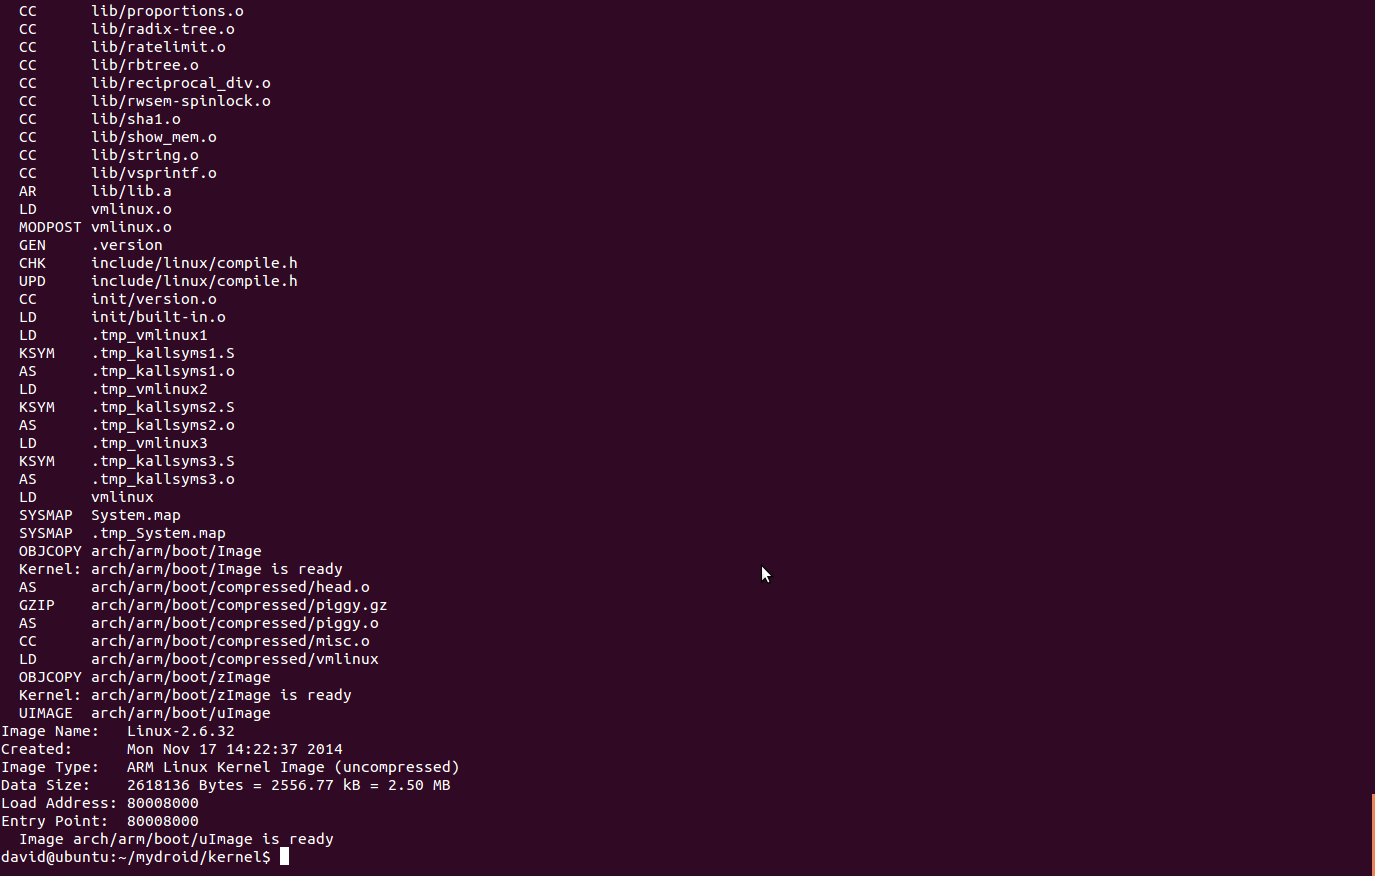
\includegraphics[width=4in]{./figs/kernel.png}
	\caption{Kernel successfully compiled}
	\label{kernel}
\end{figure}


\subsection{Build Boot Loader}
We change directory to `$\sim$/mydroid/uboot'. Similar to kernel compilaton, three steps are required:

\begin{lstlisting}[language={make}]
make CROSS_COMPILE=arm-eabi- distclean
make CROSS_COMPILE=arm-eabi- omap3_beagle_config
make CROSS_COMPILE=arm-eabi-
\end{lstlisting}

It should take less than 5 minutes and 'u-boot.bin' will be generated under the current directory. We list in Fig. \ref{uboot} compiling information for reference.

\begin{figure}[ht]
	\centering
	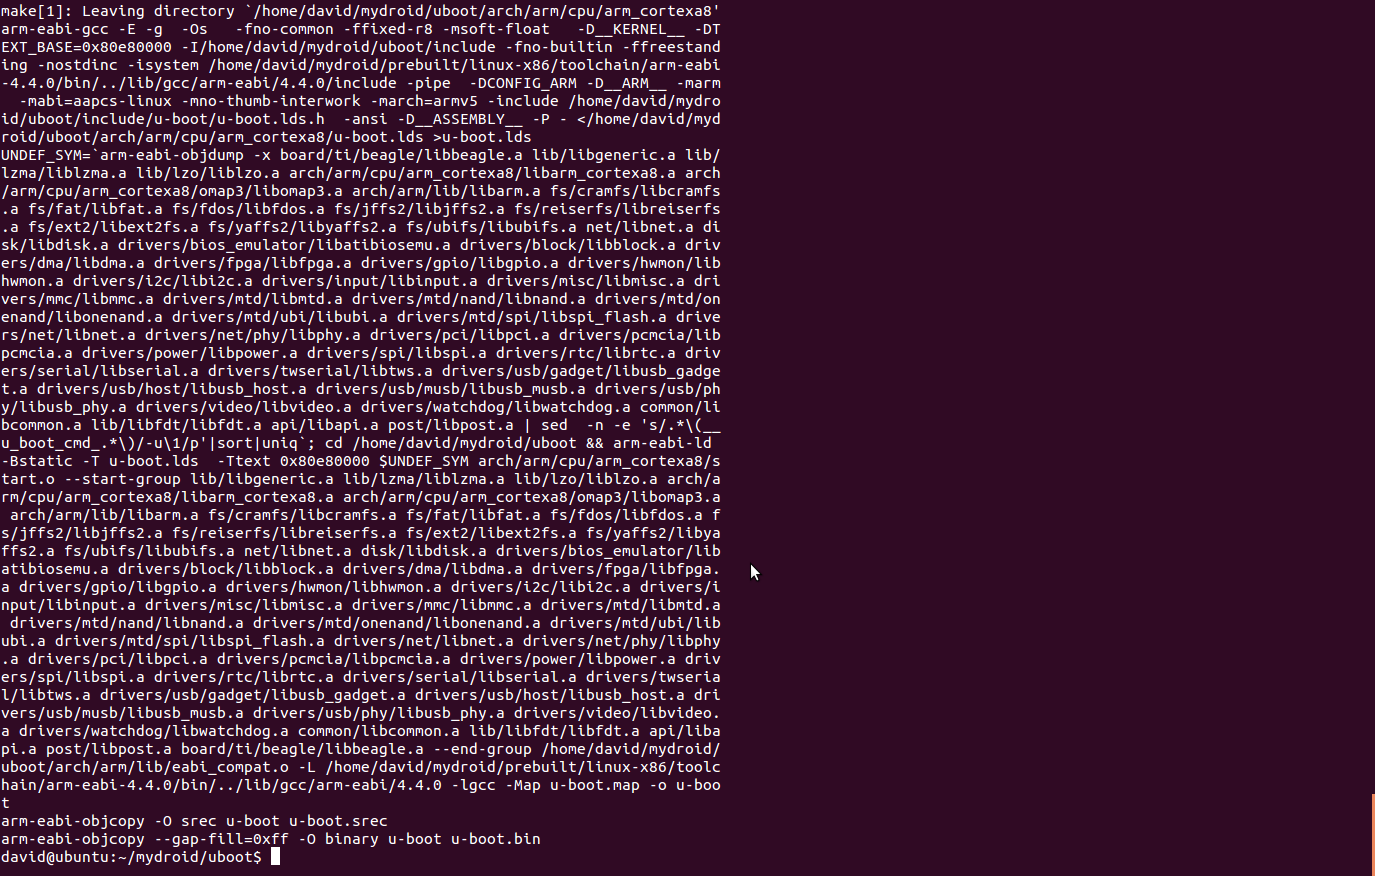
\includegraphics[width=4in]{./figs/uboot.png}
	\caption{U-boot successfully compiled}
	\label{uboot}
\end{figure}


\subsection{Build x-loader}
From the `mydroid' sources directory

\begin{lstlisting}[language={bash}]
cd ~/mydroid/x-loader
\end{lstlisting}

Execute the following commands to the kernel sources

\begin{lstlisting}[language={make}]
make CROSS_COMPILE=arm-eabi- distclean
make CROSS_COMPILE=arm-eabi- omap3beagle_config
make CROSS_COMPILE=arm-eabi-
\end{lstlisting}

This leads to the x-loader Image `x-load.bin' shown in Fig. \ref{x-loader}

\begin{figure}[ht]
	\centering
	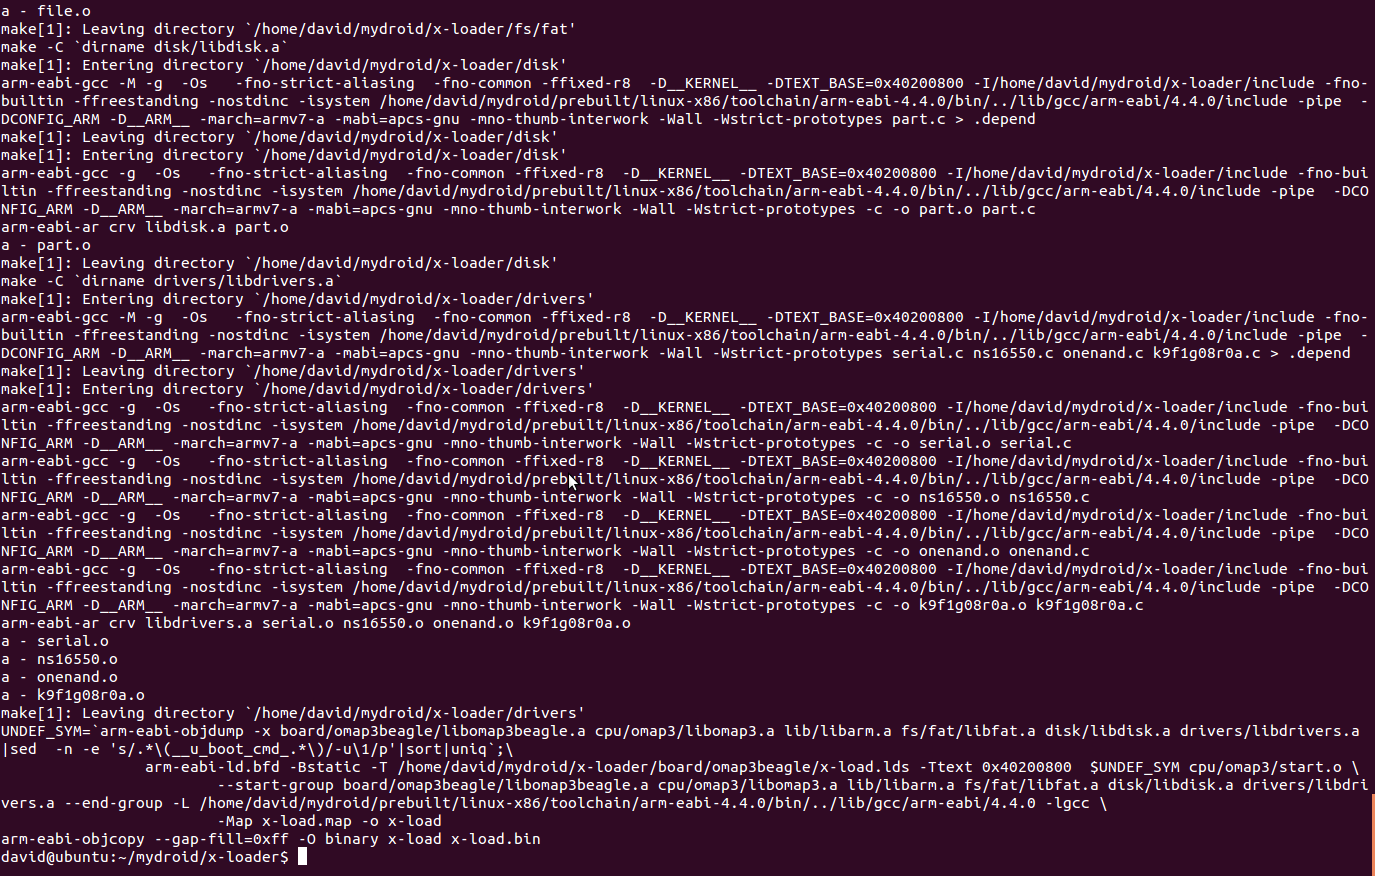
\includegraphics[width=4in]{./figs/x-loader.png}
	\caption{X-loader successfully compiled}
	\label{x-loader}
\end{figure}

To create the MLO file used for booting from a MMC/SD card, sign the x-loader image using the signGP tool found
in the Tools directory of the Devkit. 

\begin{lstlisting}[language={bash}]
../../Tools/signGP/signGP ./x-load.bin
\end{lstlisting}

The signGP tool will create a x-loader.bin.ift file, that can be renamed to MLO.

\subsection{Build boot.scr}
boot.scr is required for booting the system, and it can be generated by mk-bootscr.
First download 'TI\_Android\_GingerBread\_2\_3\_4\_DevKit\_2\_1' which has been provided in the Win7 sharefolder.
Then execute the following commands:
\begin{lstlisting}[language={bash}]
cd TI_Android_GingerBread_2_3_4_DevKit_2_1/TI_Android_GingerBread_2_3_4_DevKit_2_1/Tools/mk-bootscr/
./bootscr
\end{lstlisting}
 
\subsection{Build Android Filesystem}
Build Android filesystem for Beaglebone-xm by doing following:

 \begin{lstlisting}[language={make}]
make TARGET_PRODUCT=beagleboard OMAPES=5.x -j8
make TARGET_PRODUCT=beagleboard droid 
\end{lstlisting}
Fig. \ref{filesystem} depicts the corresponding messages from the terminal.
\begin{figure}[ht]
	\centering
	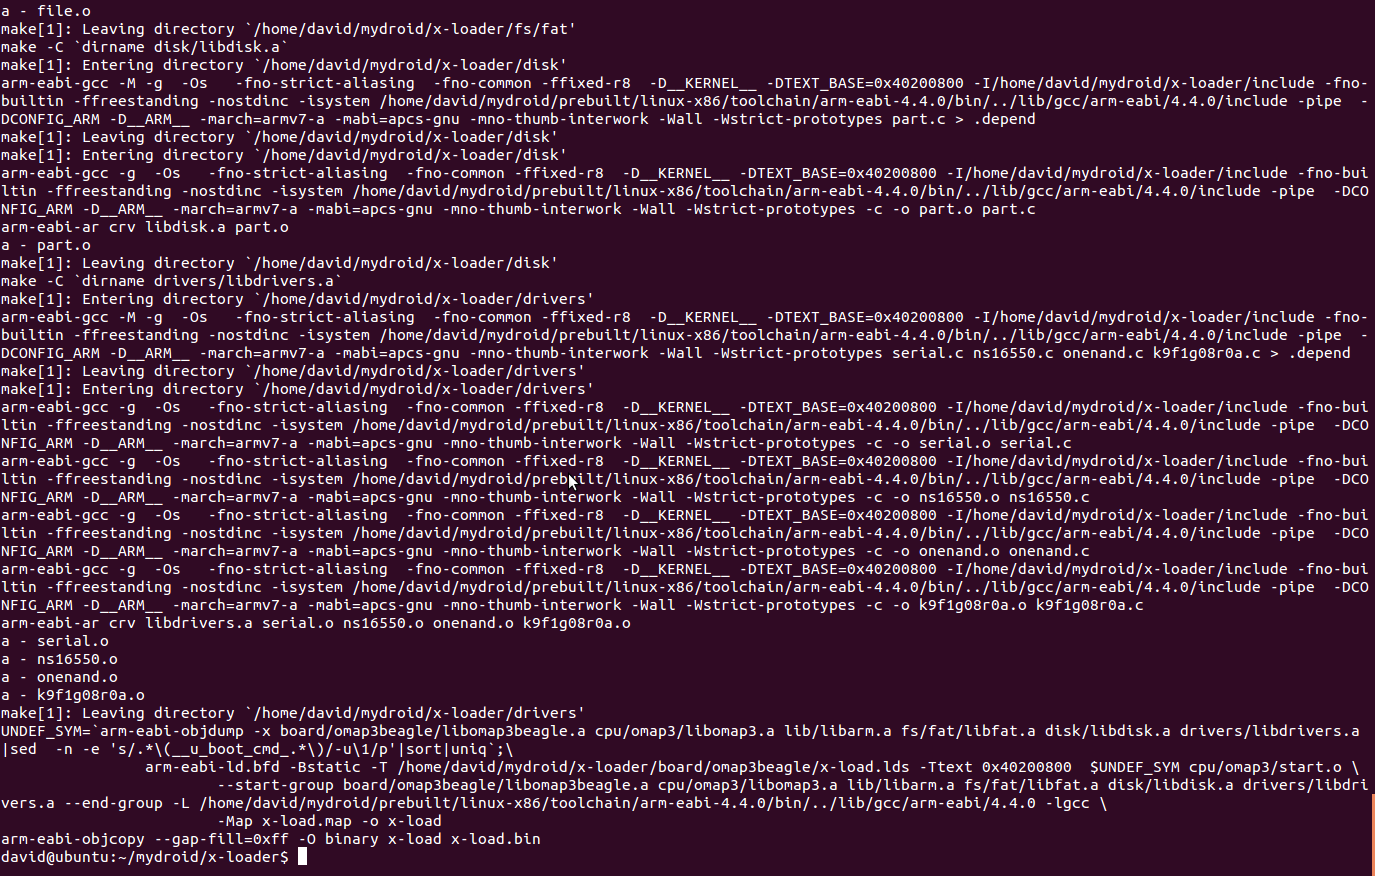
\includegraphics[width=4in]{./figs/x-loader.png}
	\caption{Filesystem successfully compiled}
	\label{filesystem}
\end{figure}

Next we compress the files generated into one single tar package. 
 \begin{lstlisting}[language={bash}]
cd out/target/product/beagleboard
cp -r root/* android_rootfs
cp -r system android_rootfs
sudo ../../../../build/tools/mktarball.sh ../../../host/linux-x86/bin/fs_get_stats android_rootfs . rootfs rootfs.tar.bz2
\end{lstlisting}
Note that rootfs.tar.bz2 is exactly the Android filesystem that we need in this experiment.

\subsection{Build OS image}
For simplicity, we rearrange those files compiled from source code into one folder `beagleboard-xm' as shown in Fig. \ref{bb-xm}.
\begin{figure}[ht]
	\centering
	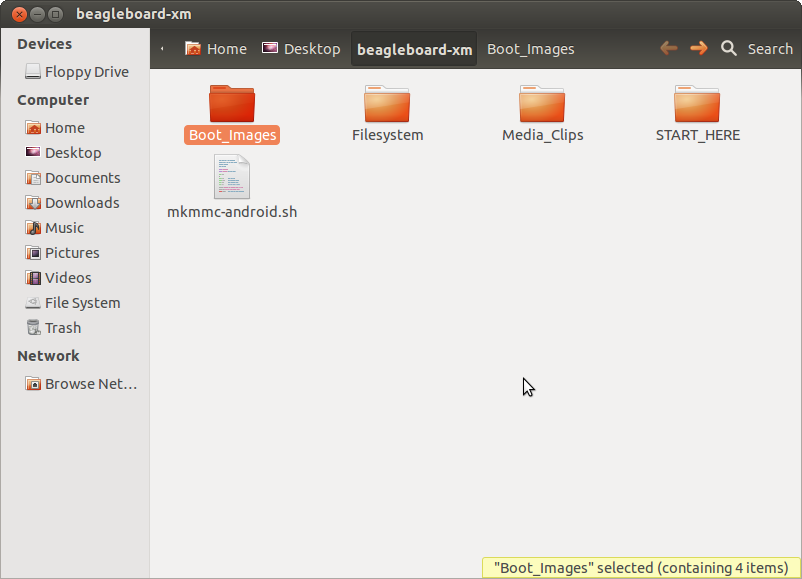
\includegraphics[width=4in]{./figs/bb-xm.png}
	\caption{Pre-built Image}
	\label{bb-xm}
\end{figure}

In the subfolder `Boot\_Images', we place boot.scr, MLO, u-boot.bin, uImage; In `Filesystem', we put  rootfs.tar.bz2; Other resources like video and pictures should be laid in `Media\_Clips', which can be found from Lab 1. The shell script 'mkmmc-android.sh' is also the same as used in Lab 1.

Insert your SD card and perform the following commands, a new image would be ready for booting. 
 \begin{lstlisting}[language={bash}]
sudo ./mkmmc-android /dev/sdb MLO u-boot.bin uImage boot.scr rootfs.tar.bz2
\end{lstlisting}

% % % % % % % % % % % % % % % % % % % % % % % % % % % % % % % % %
% % % % % % % % % % % % % % % % % % % % % % % % % % % % % % % % %
\section{Install and uninstall applications}\label{HdDes}

BBB is a low-cost, community-supported hardware device for embedded application development. BBB board mainly contains an ARM Cortex A8 series processor, a 512MB DDR3 RAM memory, an onboard 2GB MMC chip, with some other necessary peripherals. In this project, the BBB board is developed with following cables and devices: 



% % % % % % % % % % % % % % % % % % % % % % % % % % % % % % % % %
% % % % % % % % % % % % % % % % % % % % % % % % % % % % % % % % %
\section{Running Applications}\label{SfDes}

In this project, the software implementation includes installation, configuration as well as application of embedded OS, Web server, PHP, and MySQL; setup and website-based control of onboard LEDs and the C920 Web Camera. Fig.\ref{sw1} provides a block diagram of software description.
	
\subsection{Wireless Adapter Configuration}\label{Wireless}
Once the OS is successfully set up on board, it becomes critical to have Internet access --- We need to install extra system utilities or download third-party libraries to support this project. So in this section, we detail how to set up a WiFi connection for BBB.


To make the modifications into effect, we type in the following command from Secure Shell Client to restart the wirless adapter:
\begin{lstlisting}[language={bash}]
ifconfig wlan0 down && ifconfig wlan0 up
\end{lstlisting}






% % % % % % % % % % % % % % % % % % % % % % % % % % % % % % % % %
% % % % % % % % % % % % % % % % % % % % % % % % % % % % % % % % %	
\section{Q\&A}\label{Con}
In this section, we answer those questions raised by the sample report.

\begin{verbatim}
>> Q1 <<
> What is the version of toolchain or gcc you are using?
\end{verbatim}
\textbf{Reply:} We can type in the terminal `which arm-eabi-gcc' to confirm the gcc version we are 
using. In this experiment, we shall obtain `arm-wabi-gcc-4.4.0'.

\begin{verbatim}
>> Q2 <<
> Why is static library and not dynamic library and so on?
\end{verbatim}
\textbf{Reply:} Dynamic library is used because we cannot ensure each host machine has 
the related .dll files for a complete compilation. 

\begin{verbatim}
>> Q3 <<
>  Explain why use objcopy?
\end{verbatim}
\textbf{Reply:} Bootloader only accepts .bin(raw binary) files, so if we just have S-record file and then 
objcopy can help convert it into a different form, e.g. .bin file.

\begin{verbatim}
>> Q4 <<
> How you make boot.src and why you need to do so.
\end{verbatim}
\textbf{Reply:} We have demonstrated how to make boot.src in section I.(E). 
boot.src is a U-Boot script. It contains instructions for U-Boot. Using these instruction, the kernel is loaded into memory, and (optionally) a ramdisk is loaded. boot.scr can also pass parameters to the kernel.

\begin{verbatim}
>> Q4 <<
> For the kernel compilation, try to explain the names marked, 
> e.g. CLEAN, HOSTCC, HOSTLD, SHIPPED, UPD, CC, AS, GEN, CHK.
\end{verbatim}
\textbf{Reply:} In fact, these are nothing but variable alias defined in the makefile under 'kernel' directory.
For example, AS indicates the specific assembler of arm-eabi-gcc-4.4.0; HOSTCC indicates the gcc preinstalled
in the host Ubuntu OS; 

% % % % % % % % % % % % % % % % % % % % % % % % % % % % % % % % %
% % % % % % % % % % % % % % % % % % % % % % % % % % % % % % % % %

%\bibliographystyle{plain}
%\bibliography{bibfile}
\clearpage


\end{document}


